\documentclass[conference]{IEEEtran}
\IEEEoverridecommandlockouts
\usepackage{cite}
\usepackage{amsmath,amssymb,amsfonts}
\usepackage{graphicx}
\usepackage{booktabs}
\usepackage{array}
\usepackage{textcomp}
\usepackage{xcolor}
\usepackage{tikz}
\usetikzlibrary{arrows.meta,positioning,shapes.geometric,calc}
\newcommand{\rmseFifteen}{0.47}
\newcommand{\rmseIdealFifteen}{0.45}
\newcommand{\crbFifteen}{0.46}
\newcommand{\rmseFive}{1.49}
\newcommand{\rmseThirty}{0.08}
\newcommand{\nodFifteen}{12.0}
\newcommand{\fftFifteen}{4.4}
\newcommand{\statFifteen}{0.73}
\newcommand{\capFifteen}{0.48}
\newcommand{\feFineFive}{395}
\newcommand{\feFineFifteen}{107}
\newcommand{\feFineThirty}{19}
\newcommand{\feCoarseFifteen}{4.1}
\newcommand{\trk}{1.58}
\newcommand{\gdopT}{91}
\newcommand{\gdopMed}{109}
\newcommand{\triTheory}{1.59}

\def\BibTeX{{\rm B\kern-.05em{\sc i\kern-.025em b}\kern-.08em T\kern-.1em E\kern-.1em X}}
\newcommand{\vect}[1]{\mathbf{#1}}

% Equation box formatting
\setlength{\fboxsep}{3.5pt}
\setlength{\fboxrule}{0.7pt}

% Space optimization for balanced conference page layout
\setlength{\textfloatsep}{7pt plus 1pt minus 1pt}
\setlength{\floatsep}{5pt plus 1pt minus 1pt}
\setlength{\intextsep}{5pt plus 1pt minus 1pt}
\setlength{\dbltextfloatsep}{7pt plus 1pt minus 1pt}
\setlength{\dblfloatsep}{5pt plus 1pt minus 1pt}

% Hyperlinks and PDF metadata for full redirection and interactivity
\usepackage[
  colorlinks=true,
  linkcolor=blue!85!black,
  citecolor=blue!85!black,
  urlcolor=blue!85!black,
  bookmarks=true,
  bookmarksnumbered=true,
  pdfstartview=FitH,
  pdftitle={Frequency-Hopping-Aware Direction Finding for UAV Telemetry Using Switched-Interferometric SDR Arrays: A Digital Twin Validation},
  pdfauthor={Abhijit Prasad Mallick, Ayush Gupta, Mansi, Nihal Prakash, Ojaswi Shrivastava}
]{hyperref}

% Match references size with the rest of the paper (normalsize)
\makeatletter
\renewenvironment{thebibliography}[1]{%
  \section*{\refname}%
  \addcontentsline{toc}{section}{\refname}%
  \normalsize\vskip 0.3\baselineskip plus 0.1\baselineskip minus 0.1\baselineskip%
  \list{\@biblabel{\@arabic\c@enumiv}}%
  {\settowidth\labelwidth{\@biblabel{#1}}%
  \leftmargin\labelwidth
  \advance\leftmargin\labelsep\relax
  \itemsep 0.18\baselineskip\relax
  \usecounter{enumiv}%
  \let\p@enumiv\@empty
  \def\theenumiv{\@arabic\c@enumiv}}%
  \let\newblock\@empty
  \sloppy\clubpenalty4000\widowpenalty4000
  \sfcode`\.=1000\relax
  \normalsize
}{%
  \def\@noitemerr{\@latex@warning{Empty `thebibliography' environment}}%
  \endlist
}
\makeatother

\begin{document}

\title{Frequency-Hopping-Aware Direction Finding for UAV Telemetry Using Switched-Interferometric SDR Arrays: A Digital Twin Validation}

\author{\IEEEauthorblockN{Abhijit Prasad Mallick, Ojaswi Shrivastava, Mansi, Nihal Prakash, and Ayush Gupta}
\IEEEauthorblockA{\textit{Department of Electronics and Communication Engineering}\\
\textit{Indian Institute of Information Technology Vadodara -- International Campus Diu (IIITV-ICD)}\\
Course EC261 (Semester Project) \quad Faculty Guide: Dr.\ Varun Kumar}}

\maketitle

\section*{Abstract}
Passive direction finding (DF) of non-cooperative UAVs must cope with frequency-hopping spread-spectrum (FHSS) telemetry that changes carrier every few milliseconds, while coherent multi-channel receivers remain too costly for most laboratories. This paper presents a digital-twin validation of a low-cost DF receiver in which a four-element uniform circular array (UCA) is time-multiplexed through an SP4T RF switch into a single SDR channel. Each burst is detected by a sliding-window power trigger, its carrier is recovered by a coarse FFT followed by a lag-$M$ differential-phase refinement, and the switched samples are de-rotated to a common time base before MUSIC processing with a per-burst wavelength. An eigenvalue-ratio gate flags unreliable bursts, and a circular Kalman filter smooths the bearing. Monte Carlo simulations show that the switched array matches an ideal four-channel coherent receiver and the Cram\'er--Rao bound for SNR $\ge 5$~dB (\rmseFifteen$^\circ$ RMSE at 15~dB), whereas omitting de-rotation leaves a $12^\circ$ error floor. Static-wavelength steering biases the 7.2~cm array by under $0.75^\circ$ but fails completely beyond about 12~cm radius. The gate detects decorrelated multipath but not fully coherent reflections. Three-station triangulation reaches \trk~m RMS position error.

\vspace{0.8ex}
\begin{IEEEkeywords}
Direction of arrival (DoA), frequency-hopping spread spectrum (FHSS), MUSIC, switched antenna array, UAV telemetry, multipath detection, software-defined radio, digital twin.
\end{IEEEkeywords}

%=====================================================================
\section{Introduction}\label{sec:intro}
Unmanned aerial vehicles (UAVs) are now widespread in commercial, industrial, and recreational use, which has created a strong demand for airspace monitoring. Unlike crewed aircraft, rogue or malfunctioning drones seldom broadcast cooperative position reports, so they must be located passively. Optical and infrared sensors degrade in poor visibility, and acoustic arrays are strongly range-limited. Passive radio-frequency (RF) direction finding instead exploits the command-and-control (C2) and telemetry emissions that the UAV must radiate.

Sub-GHz links in the 433~MHz, 868~MHz, and 902--928~MHz ISM bands are attractive for this purpose. Their long wavelength (32.8~cm at 915~MHz) gives lower free-space path loss than 2.4/5.8~GHz video links, better diffraction around buildings, and lower attenuation through vegetation \cite{itu833}. It also relaxes antenna placement tolerances, and the narrow channels suit ultra-low-cost receivers such as the RTL-SDR.

The difficulty is that modern long-range links, such as ExpressLRS \cite{elrs} and SiK telemetry, use FHSS to resist interference. The emission is therefore a train of 1--5~ms packet bursts whose carrier frequency, and hence wavelength, changes from burst to burst. Classical subspace estimators such as MUSIC \cite{schmidt} and ESPRIT \cite{roy} build their steering vectors for one fixed carrier and do not account for this.

A second difficulty is cost. Multi-channel phase-coherent SDR testbeds cost on the order of \mbox{Rs.\,2~lakh}. A single receiver fed by an electronic antenna switch is far cheaper, but the antennas are then sampled one after another, so a frequency offset turns into a spurious inter-element phase rotation. Finally, reflections from concrete and scattering from foliage corrupt the spatial covariance matrix.

Because component lead times and budget prevent a hardware build at this stage, we develop and validate the complete system as a physics-based digital twin. The main contributions are:
\begin{itemize}
\item a per-burst DSP chain (power trigger, coarse FFT, lag-$M$ frequency refinement, switched-array de-rotation, and wavelength-aware MUSIC) for single-receiver FHSS direction finding;
\item an analysis of when frequency-aware steering matters, showing that it is a minor correction for the compact prototype but critical for larger apertures;
\item an honest assessment of an eigenvalue-ratio reliability gate, including its closed-form threshold behavior and its blind spot for coherent multipath;
\item Monte Carlo, tracking, and triangulation results, and a Rs.\,1{,}700 hardware roadmap.
\end{itemize}
Section~\ref{sec:gaps} states the gaps, Sections~\ref{sec:model}--\ref{sec:pipeline} the model and pipeline, Section~\ref{sec:twin} the twin, Sections~\ref{sec:setup}--\ref{sec:results} the experiments, and Sections~\ref{sec:roadmap}--\ref{sec:conclusion} the roadmap and conclusions.

%=====================================================================
\section{Problem Statement and Literature Gaps}\label{sec:gaps}
\subsection{Gap 1: Frequency-Dependent Manifold Mismatch}
Standard DoA estimators fix the carrier $f_0$ in the steering vector, but FHSS links change it every few milliseconds, so the assumed and true array manifolds differ after each hop.

\subsection{Gap 2: Hardware Cost versus Coherence}
Coherent multi-channel SDRs are expensive, while a single-receiver switched array is cheap but suffers temporal phase rotation across antenna dwell slots that ordinary receivers cannot remove.

\subsection{Gap 3: Urban Multipath and Foliage}
Concrete reflections and canopy scattering (ITU-R P.833 \cite{itu833}) add partially coherent copies that corrupt the covariance, and low-cost systems rarely include a statistical reliability check.

%=====================================================================
\section{System and Signal Model}\label{sec:model}
\subsection{FHSS Burst Model}
The $k$-th burst is a narrowband signal $s_k(t)$ transmitted at carrier $f_k \in \mathcal{F}=\{433,\,868,\,902,\,915,\,928\}$~MHz and lasting 1--5~ms. The receiver LO is tuned to the channel center $f_{\rm LO}$, so the baseband signal carries a residual offset $f_\Delta = f_k - f_{\rm LO}$ caused by oscillator error and channel mismatch.

\subsection{Uniform Circular Array Manifold}
For $M=4$ monopoles on a circle of radius $r=7.2$~cm at angles $\phi_m = 2\pi m/M$, the steering vector for azimuth $\theta$ at carrier $f$ is
\begin{equation}
\boxed{a_m(f,\theta)=\exp\!\Big(j\,\tfrac{2\pi f}{c}\,r\cos(\theta-\phi_m)\Big)},\quad m=0,\dots,M-1,
\label{eq:steer}
\end{equation}
where $c$ is the speed of light, $r$ the array radius, and $\theta$ the azimuth of arrival. The electrical radius $\kappa=2\pi f r/c$ rises from 0.65 at 433~MHz to 1.40 at 928~MHz.

\subsection{Switched Acquisition}
An SP4T switch connects element $m(n)=n \bmod M$ to the single receiver during sample $n$, so the received sequence is
\begin{equation}
\boxed{y[n]=a_{m(n)}(f_k,\theta)\,s[n]\,e^{j2\pi f_\Delta nT_s}+w[n]},
\label{eq:switched}
\end{equation}
where $s[n]$ is the complex burst envelope, $T_s=1/f_s$ the sample period, and $w[n]\sim\mathcal{CN}(0,\sigma^2)$ white noise. The factor $e^{j2\pi f_\Delta nT_s}$ is the phase rotation that a conventional receiver would misread as spatial phase.

\subsection{Two-Path Channel}
To model a reflection or foliage-scattered path we add a second path from azimuth $\theta_r$:
\begin{equation}
y_{\rm mp}[n]=y[n]+\rho\,e^{j\psi}a_{m(n)}(f_k,\theta_r)\,s_r[n]\,e^{j2\pi f_\Delta nT_s},
\label{eq:mp}
\end{equation}
\begin{equation}
s_r[n]=c\,s[n]+\sqrt{1-|c|^2}\,s'[n],
\label{eq:corr}
\end{equation}
where $\rho$ is the reflected-to-direct amplitude ratio, $\psi$ a random path phase, $s'[n]$ an independent copy of the signal, and $c\in[0,1]$ the correlation coefficient between the two paths. A value $c=1$ is a perfectly coherent specular reflection, and $c=0$ is a fully decorrelated one. Vegetation attenuation \cite{itu833} lowers $\rho$, while scatterer motion lowers $c$.

%=====================================================================
\section{Proposed DSP Pipeline}\label{sec:pipeline}
Fig.~\ref{fig:block} summarizes the processing chain, which runs once per received burst of $N=256$ samples.

\begin{figure*}[!t]
\centering
\resizebox{\textwidth}{!}{%
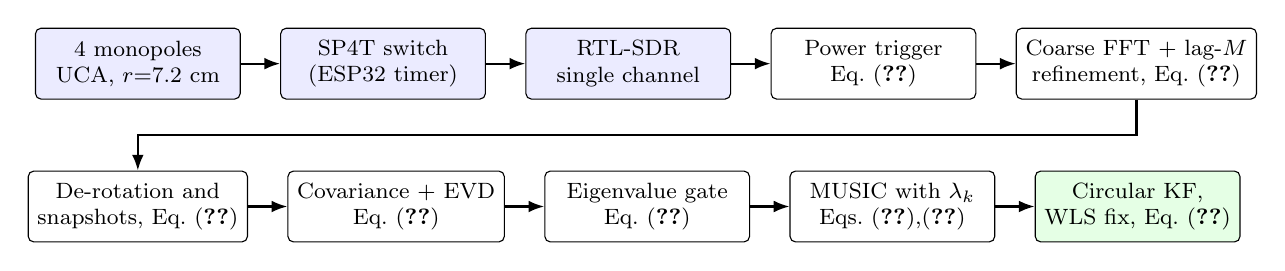
\begin{tikzpicture}[font=\footnotesize, node distance=5mm,
  blk/.style={draw, rounded corners=2pt, minimum height=9mm, minimum width=26mm, align=center, fill=gray!8},
  rf/.style={blk, fill=blue!8},
  dsp/.style={blk, fill=white},
  outb/.style={blk, fill=green!10},
  ar/.style={-{Latex[length=2mm]}, thick}]
\node[rf] (a) {4 monopoles\\UCA, $r{=}7.2$ cm};
\node[rf, right=of a] (b) {SP4T switch\\(ESP32 timer)};
\node[rf, right=of b] (c) {RTL-SDR\\single channel};
\node[dsp, right=of c] (d) {Power trigger\\Eq.~(\ref{eq:trig})};
\node[dsp, right=of d] (e) {Coarse FFT $+$ lag-$M$\\refinement, Eq.~(\ref{eq:fine})};
\node[dsp, below=9mm of a] (f) {De-rotation and\\snapshots, Eq.~(\ref{eq:derot})};
\node[dsp, right=of f] (g) {Covariance $+$ EVD\\Eq.~(\ref{eq:cov})};
\node[dsp, right=of g] (h) {Eigenvalue gate\\Eq.~(\ref{eq:gate})};
\node[dsp, right=of h] (i) {MUSIC with $\lambda_k$\\Eqs.~(\ref{eq:lam}),(\ref{eq:music})};
\node[outb, right=of i] (j) {Circular KF,\\WLS fix, Eq.~(\ref{eq:kf})};
\foreach \s/\t in {a/b,b/c,c/d,d/e,f/g,g/h,h/i,i/j} \draw[ar] (\s) -- (\t);
\draw[ar] (e.south) -- ++(0,-4.5mm) -| ($(f.north)+(0,4.5mm)$) -- (f.north);
\end{tikzpicture}}
\caption{Block diagram of the proposed switched-array DF receiver. Blue blocks are hardware; white blocks are per-burst DSP stages; the green block is the tracking and localization back end.}
\label{fig:block}
\end{figure*}

\subsection{Burst Detection}
A sliding-window power detector isolates bursts without clock synchronization:
\begin{equation}
\boxed{P[n]=\frac{1}{W}\sum_{k=0}^{W-1}\left|y[n-k]\right|^2},
\label{eq:trig}
\end{equation}
where $W$ is the window length. A burst is declared when $P[n]>\eta$ (here $\eta=0.07$ in normalized units), and the burst samples are cut out for further processing.

\subsection{Carrier Recovery}
A Hann-windowed $N$-point FFT, searched only in $|f|<f_s/(2M)$, gives a coarse offset $f_c$. Because the antenna switch imposes a phase jump on every sample, we refine with a lag-$M$ differential-phase estimator in the Kay/Fitz family \cite{kay,fitz}, which compares samples from the \emph{same} element so the switching phase cancels:
\begin{equation}
\boxed{\hat f_\Delta=f_c+\frac{f_s}{2\pi M}\arg\!\Big(\sum_{n=M}^{N-1}\tilde y[n]\,\tilde y^{*}[n-M]\Big)},
\label{eq:fine}
\end{equation}
where $\tilde y[n]=y[n]e^{-j2\pi f_cnT_s}$ is the coarsely corrected sequence and $(\cdot)^*$ denotes conjugation. The estimate is unambiguous for $|f_\Delta|<f_s/(2M)$. The carrier and wavelength then follow as
\begin{equation}
\boxed{f_{\rm RF}=f_{\rm LO}+\hat f_\Delta,\qquad \lambda_k=\frac{c}{f_{\rm RF}}}.
\label{eq:lam}
\end{equation}

\subsection{De-rotation and Snapshot Formation}
Removing the estimated rotation places all elements on a common time base:
\begin{equation}
\begin{gathered}
\boxed{x[n]=y[n]\,e^{-j2\pi\hat f_\Delta nT_s}},\\
\vect{x}_q=\big[x[qM],\dots,x[qM{+}M{-}1]\big]^{T},
\end{gathered}
\label{eq:derot}
\end{equation}
where $\vect{x}_q$ is the $q$-th snapshot, $q=0,\dots,K{-}1$, and $K=N/M=64$.

\subsection{Covariance and Eigendecomposition}
The sample covariance is eigendecomposed (cyclic Jacobi) into signal and noise parts:
\begin{equation}
\boxed{\hat{\vect{R}}=\frac{1}{K}\sum_{q=0}^{K-1}\vect{x}_q\vect{x}_q^{H}=\vect{E}_s\boldsymbol{\Lambda}_s\vect{E}_s^{H}+\vect{E}_n\boldsymbol{\Lambda}_n\vect{E}_n^{H}},
\label{eq:cov}
\end{equation}
where $\vect{E}_s$ and $\vect{E}_n$ span the signal and noise subspaces and $\boldsymbol{\Lambda}_{s,n}$ hold the eigenvalues $\lambda_1\ge\dots\ge\lambda_M$.

\subsection{Eigenvalue Reliability Gate}
A burst is accepted only if the dominant eigenvalue clearly separates from the second:
\begin{equation}
\boxed{\gamma=\frac{\lambda_1}{\lambda_2}\ \mathop{\gtrless}_{\text{REJECT}}^{\text{ACCEPT}}\ \gamma_{\rm th}=8}.
\label{eq:gate}
\end{equation}
With per-element SNR $\Gamma$ and $\sigma^2=1$, a clean line-of-sight burst gives $\gamma\approx M\Gamma+1$, so the gate also rejects bursts below $\Gamma\approx 2.4$~dB. For two uncorrelated paths with nearly orthogonal steering vectors,
\begin{equation}
\gamma\approx\frac{M\Gamma+1}{M\Gamma\rho^{2}+1}\ \xrightarrow{\ \Gamma\gg1\ }\ \frac{1}{\rho^{2}},
\label{eq:gamma}
\end{equation}
so $\gamma_{\rm th}=8$ corresponds to rejecting reflections stronger than $\rho^2=1/8$ ($-9$~dB). As $|c|\to1$ the covariance returns to rank one and $\gamma$ grows again, which is the gate's fundamental limit.

\subsection{MUSIC and Circular Kalman Filter}
With $\vect{E}_n=[\vect{v}_2,\dots,\vect{v}_M]$, the pseudospectrum uses the per-burst wavelength through $a_m(f_{\rm RF},\theta)$:
\begin{equation}
\boxed{P_{\rm MUSIC}(\theta)=\frac{1}{\vect{a}^{H}(f_{\rm RF},\theta)\,\vect{E}_n\vect{E}_n^{H}\,\vect{a}(f_{\rm RF},\theta)}},
\label{eq:music}
\end{equation}
and the peak is refined by parabolic interpolation on a $0.1^\circ$ grid. Accepted bearings $z$ drive a Kalman filter on state $[\theta,\omega]^T$ (bearing and rate) whose innovation is wrapped to $\pm180^\circ$:
\begin{equation}
\boxed{\theta^{+}=\theta^{-}+K_g\,\nu},
\label{eq:kf}
\end{equation}
where $\theta^-$ is the predicted bearing, $K_g$ the Kalman gain, and the innovation is wrapped via $\nu=\big((z-\theta^{-}+180^\circ)\bmod 360^\circ\big)-180^\circ$. Rejected bursts only run the prediction step (hold-track).

\subsection{Performance Bound}
For a single source, the deterministic Cram\'er--Rao bound on $\theta$ is \cite{stoica}
\begin{equation}
\boxed{\mathrm{CRB}(\theta)=\frac{\sigma^2}{2KP_s\Big[\dot{\vect a}^{H}\dot{\vect a}-\dfrac{|\vect a^{H}\dot{\vect a}|^2}{\vect a^{H}\vect a}\Big]}},
\label{eq:crb}
\end{equation}
where $P_s$ is the signal power, $K$ the snapshot count, and $\dot{\vect a}=\partial\vect a/\partial\theta$.

%=====================================================================
\section{Digital Twin Architecture}\label{sec:twin}
The twin is organized into four coupled workspaces, providing the comprehensive physical and digital signal processing simulation suite illustrated in Fig.~\ref{fig:dashboard}.

\begin{figure*}[!t]
\centering
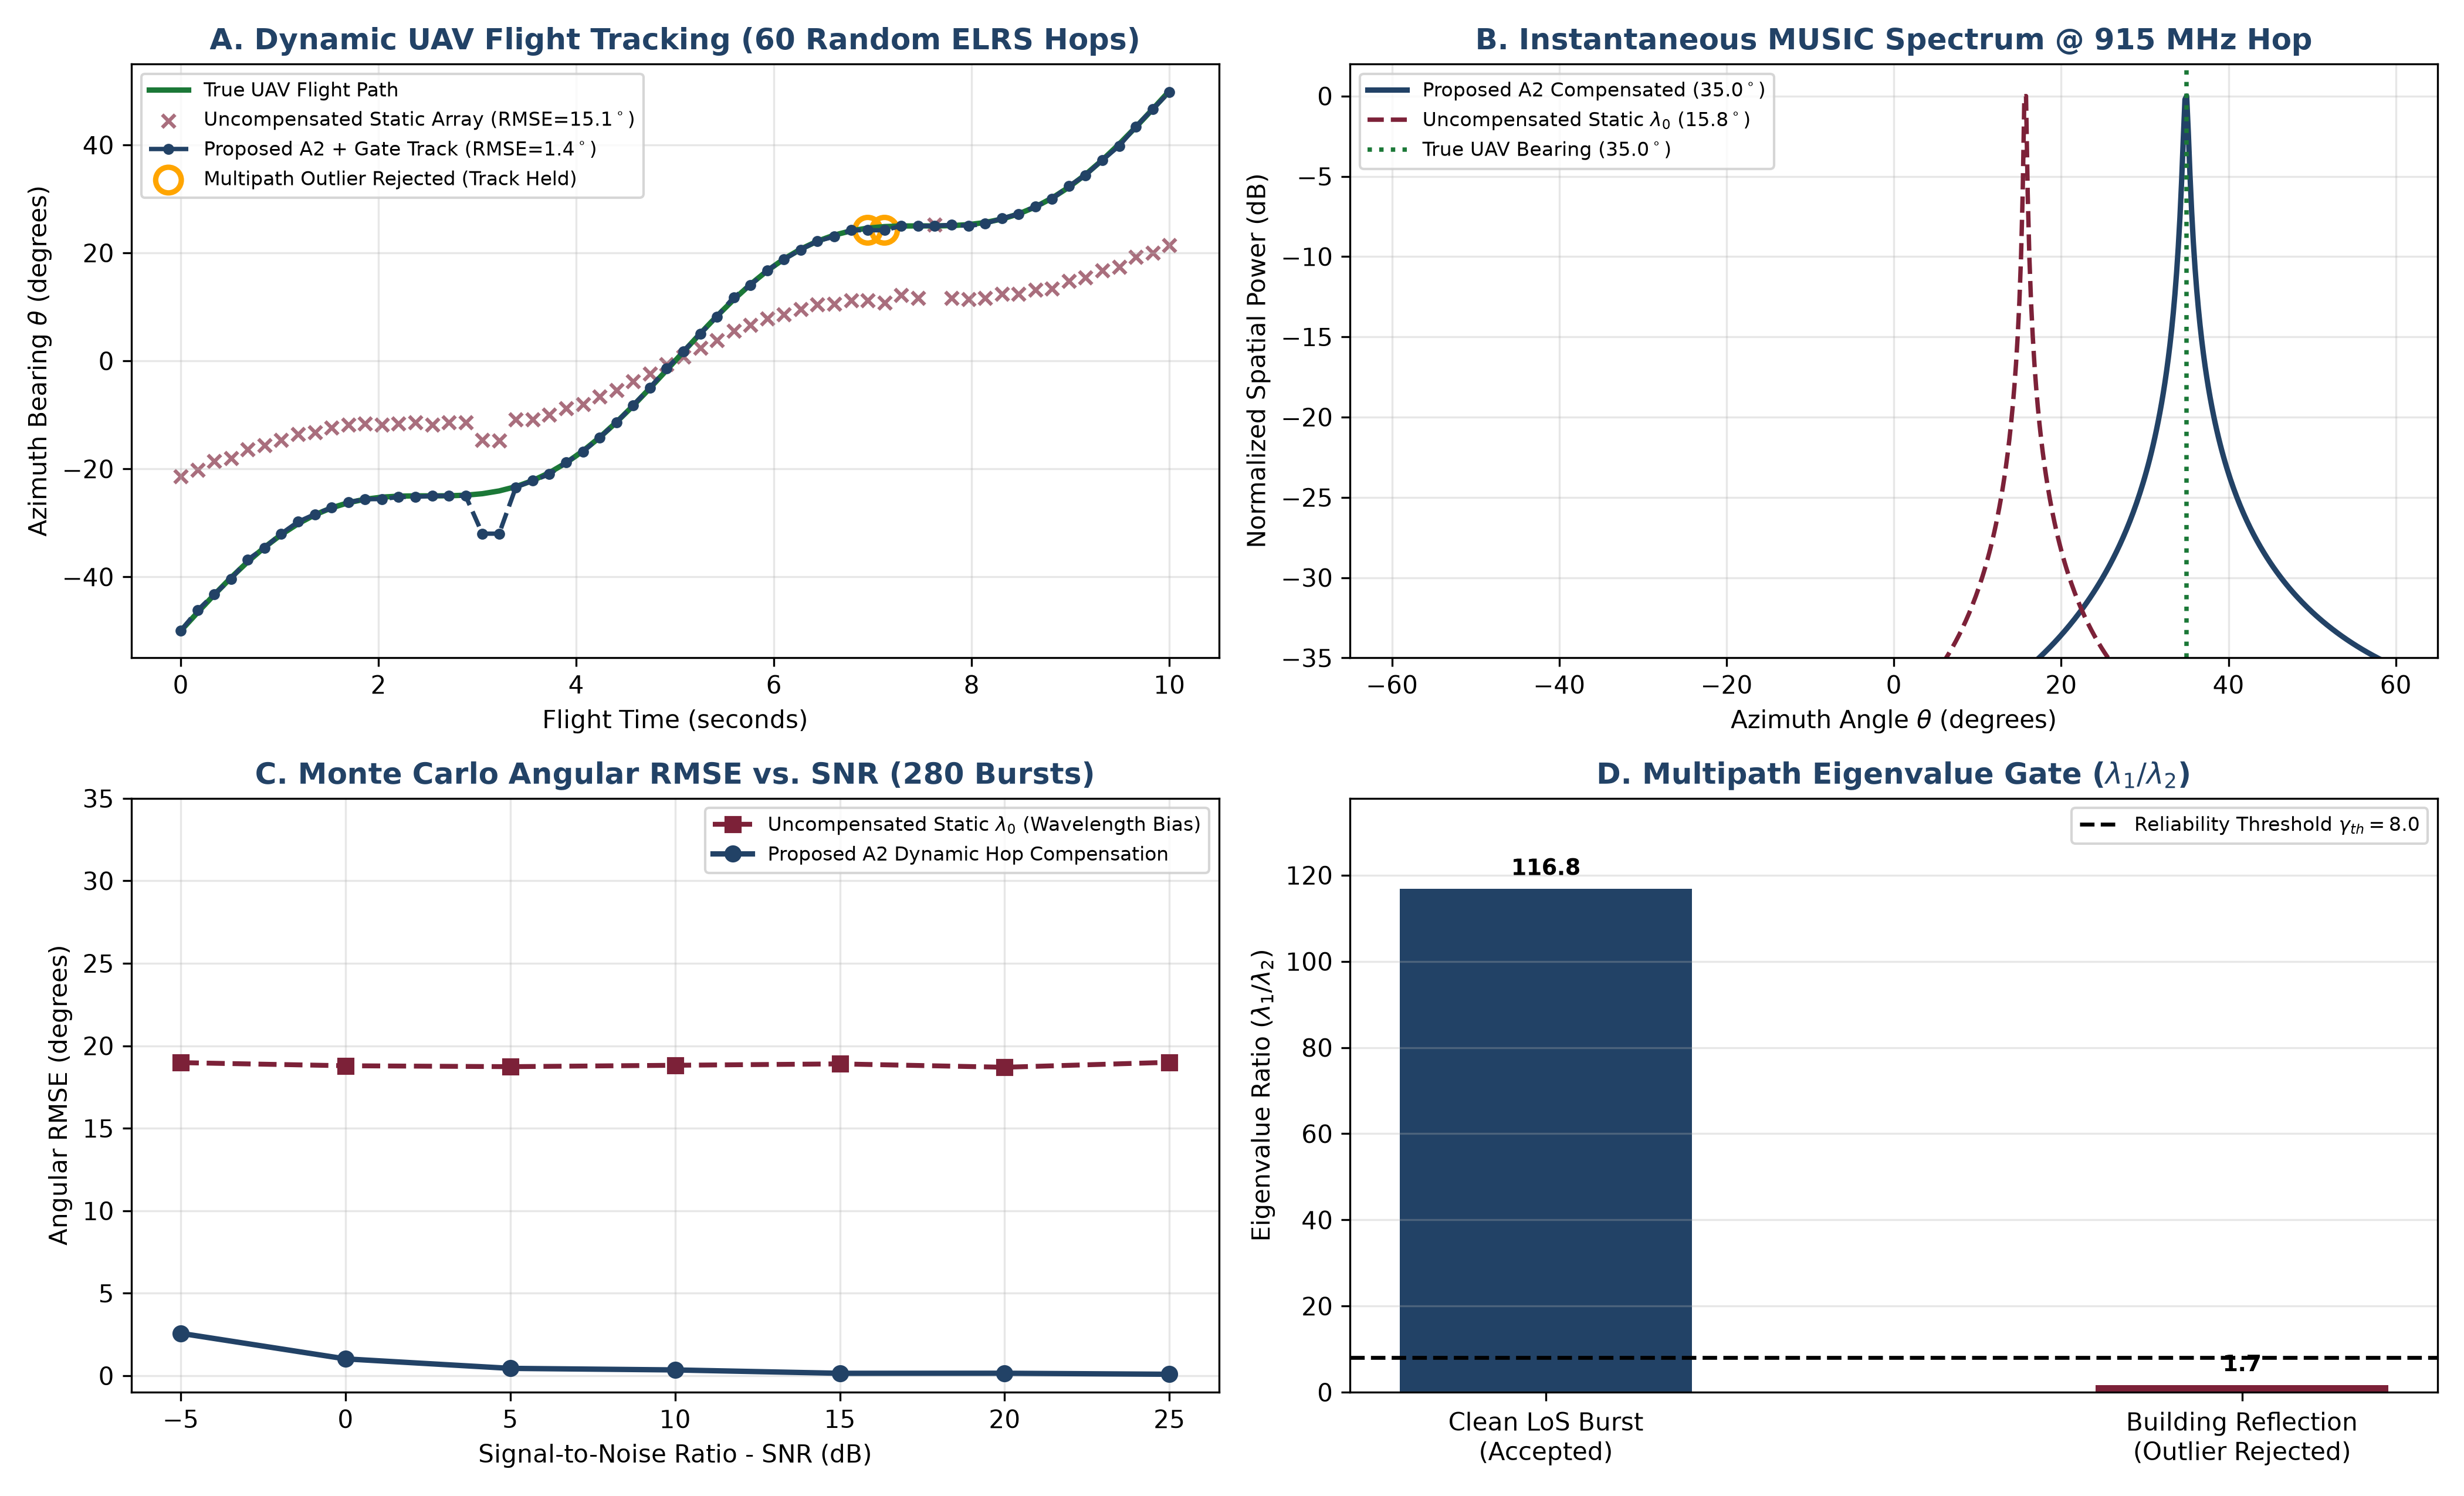
\includegraphics[width=\textwidth]{figs/fig_dashboard.png}
\caption{The developed EC261 UAV RF Direction Finding Digital Twin simulation dashboard: (a) Dynamic UAV flight tracking across 60 random ELRS hops comparing the proposed A2 gated track (RMSE = $1.4^\circ$) against the uncompensated static array (RMSE = $15.1^\circ$); (b) Instantaneous MUSIC spatial pseudospectrum at 915~MHz hop; (c) Monte Carlo angular RMSE versus SNR across 280 bursts; (d) Multipath eigenvalue ratio gate ($\lambda_1/\lambda_2$) showing successful outlier rejection of building multipath reflection.}
\label{fig:dashboard}
\end{figure*}

\subsection{Mission Control (3D Arena)}
A three-dimensional tactical arena of $120\times120$~m models concrete blocks, forest regions with ITU-R P.833 foliage \cite{itu833}, and a UAV flying 3D trajectories while emitting FHSS bursts. Four camera presets (isometric, top-down, array zoom, follow) and Forest, Urban, and Mixed environment modes are provided, together with a material-wave inspector that shows the seven-component ray bundle and Snell refraction at each surface.

\subsection{Signal Analysis Lab}
An oscilloscope-style workspace plots the power envelope, FFT bins, MUSIC pseudospectra (compensated versus static), and covariance eigenvalues for every burst.

\subsection{Experiment Lab}
A Monte Carlo harness sweeps SNR from $-10$ to $+30$~dB and benchmarks the estimators automatically. The results of Section~\ref{sec:results} were produced with a NumPy implementation of the same equations.

\subsection{EM Maxwell Lab}
This workspace hosts a 2D/3D finite-difference time-domain (FDTD) solver on a Yee grid \cite{yee} for visual inspection of reflection and scattering geometry, and a three-station bearing-only localizer. With bearings $\theta_i$ from stations at $\vect{p}_i$, the weighted least-squares fix and its dilution of precision are
\begin{equation}
\boxed{\hat{\vect p}=\arg\min_{\vect p}\sum_{i=1}^{3}\frac{\big[\theta_i-\operatorname{atan2}(\vect p-\vect p_i)\big]^2}{\sigma_i^2}},
\label{eq:wls}
\end{equation}
\begin{equation}
\boxed{\mathrm{GDOP}=\sqrt{\operatorname{tr}\big[(\vect H^{T}\vect H)^{-1}\big]}},
\label{eq:gdop}
\end{equation}
where $\sigma_i$ is the bearing standard deviation at station $i$ and $\vect H$ is the Jacobian of the bearings with respect to position \cite{torrieri}. Only the localizer is used for quantitative results here; the FDTD module is not evaluated in this paper.

%=====================================================================
\section{Simulation Setup}\label{sec:setup}
Table~\ref{tab:params} lists the parameters. Each burst is a BPSK-modulated narrowband signal sampled at 250~kS/s (a 1.02~ms burst, within the 1--5~ms range). Bursts are assumed to be correctly segmented, so the trigger of Eq.~(\ref{eq:trig}) is not exercised in the Monte Carlo runs. Switching is sample-synchronous, and the SNR is defined per element and per sample. Azimuths are drawn uniformly unless stated otherwise.

\begin{table}[!t]
\caption{Simulation Parameters}
\label{tab:params}
\centering
\small
\begin{tabular}{@{}ll@{}}
\toprule
Parameter & Value \\
\midrule
Array & UCA, $M=4$, $r=7.2$~cm, ideal monopoles \\
Hop set $\mathcal F$ & 433, 868, 902, 915, 928 MHz \\
Sample rate $f_s$ & 250 kS/s ($N=256$, $K=64$ snapshots) \\
Residual offset $f_\Delta$ & uniform in $\pm20$ kHz \\
Symbol length & 16 samples (64 $\mu$s), BPSK \\
Gate threshold $\gamma_{\rm th}$ & 8.0 \\
Trials per point & 400 (SNR sweep), 600--1000 (tables) \\
Static reference $f_0$ & 433 MHz \\
\bottomrule
\end{tabular}
\end{table}

%=====================================================================
\section{Results and Discussion}\label{sec:results}
\begin{figure*}[!t]
\centering
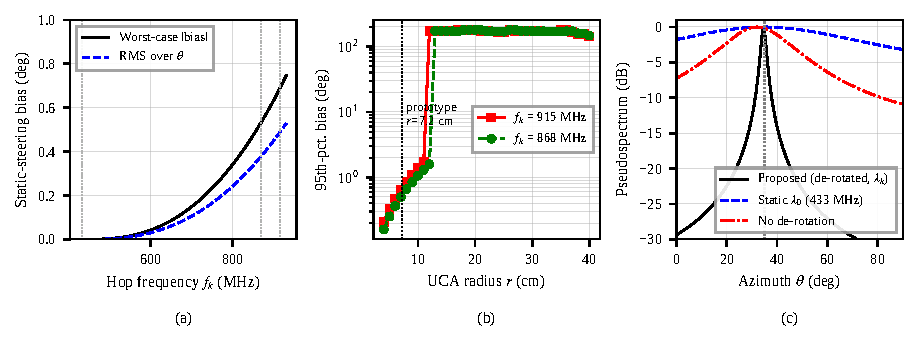
\includegraphics[width=\textwidth]{figs/fig_bias.pdf}
\caption{Manifold mismatch analysis. (a) Bias of MUSIC with static 433~MHz steering versus hop frequency ($r=7.2$~cm). (b) 95th-percentile bias versus UCA radius. (c) Pseudospectra for a 915~MHz burst at 35$^\circ$ and 15~dB SNR.}
\label{fig:bias}
\end{figure*}
\begin{figure*}[!t]
\centering
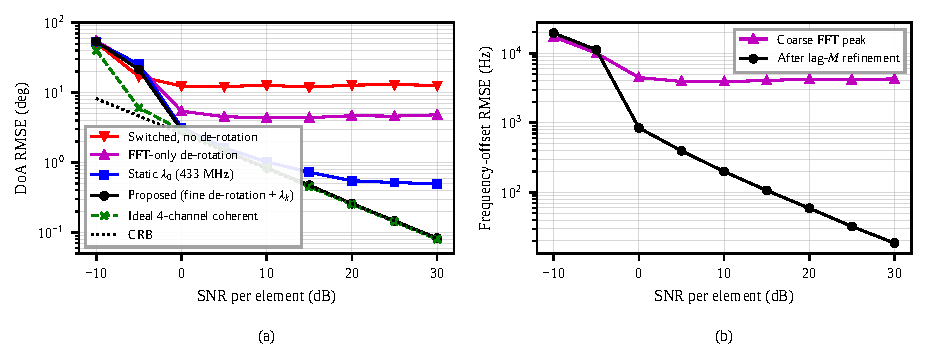
\includegraphics[width=\textwidth]{figs/fig_rmse.pdf}
\caption{(a) DoA RMSE versus SNR at 915~MHz for receiver variants, the ideal coherent four-channel baseline, and the CRB. (b) Frequency-offset RMSE before and after lag-$M$ refinement.}
\label{fig:rmse}
\end{figure*}
\subsection{Effect of FHSS Manifold Mismatch}
Fig.~\ref{fig:bias}(a) shows the noiseless MUSIC bias when a static steering vector calibrated at 433~MHz is applied to hopped bursts. For the 7.2~cm array the bias stays below $0.75^\circ$ across 430--930~MHz. The reason is geometric: for $M=4$ the element phases are $\pm\kappa\cos\theta$ and $\pm\kappa\sin\theta$, so a wrong wavelength rescales $\kappa$ but leaves the direction $\theta$ nearly unchanged. Table~\ref{tab:hops} confirms this: the static bias at 915~MHz is only $0.46^\circ$, against $0.01^\circ$ for the proposed method.


\begin{table}[!t]
\caption{FHSS Benchmark: $\theta_{\rm true}=35^\circ$, SNR $=15$~dB (Degrees)}
\label{tab:hops}
\centering
\small
\begin{tabular}{@{}cccccc@{}}
\toprule
 & & \multicolumn{2}{c}{Static $\lambda_0$} & \multicolumn{2}{c}{Proposed} \\
\cmidrule(lr){3-4}\cmidrule(lr){5-6}
$f_k$ (MHz) & $\kappa$ & Bias & RMSE & Bias & RMSE \\
\midrule
433.0 & 0.65 & +0.02 & 0.97 & +0.02 & 0.97 \\
868.0 & 1.31 & +0.32 & 0.61 & 0.00 & 0.50 \\
902.0 & 1.36 & +0.43 & 0.67 & +0.01 & 0.47 \\
915.0 & 1.38 & +0.46 & 0.66 & +0.01 & 0.46 \\
928.0 & 1.40 & +0.46 & 0.66 & $-$0.03 & 0.44 \\
\bottomrule
\end{tabular}
\end{table}

Mismatch does, however, flatten the pseudospectrum: in Fig.~\ref{fig:bias}(c) and Fig.~\ref{fig:dashboard}(b), the peak-to-median contrast falls from 34.1~dB (proposed) to 4.9~dB (static), which reduces confidence and resolvability even though the peak position is nearly correct. Fig.~\ref{fig:bias}(b) shows the strong dependence on aperture: the bias remains near $1^\circ$ up to $r\approx 11$~cm, then jumps to about $170^\circ$ (an ambiguity failure) for $r\gtrsim12$~cm at 915~MHz. FHSS-aware steering is therefore a refinement for the compact prototype but essential for larger arrays. At 433~MHz the RMSE is higher (0.97$^\circ$) simply because the electrical aperture is smaller.

\subsection{Switched-Array De-rotation and Bound}
Fig.~\ref{fig:rmse}(a) compares receiver variants at 915~MHz. Without de-rotation the RMSE saturates near $12^\circ$ regardless of SNR, because the switching rotation is read as spatial phase. De-rotating with only the coarse FFT estimate leaves a floor of $\fftFifteen^\circ$ at 15~dB: the bursts are modulated, so the FFT peak is accurate only to about \feCoarseFifteen~kHz (Fig.~\ref{fig:rmse}(b)). The lag-$M$ refinement lowers the frequency error to \feFineFifteen~Hz at 15~dB, and the proposed receiver reaches \rmseFifteen$^\circ$ RMSE, compared with \rmseIdealFifteen$^\circ$ for an ideal four-channel coherent receiver and a CRB of \crbFifteen$^\circ$. At 5 and 30~dB the proposed RMSE is \rmseFive$^\circ$ and \rmseThirty$^\circ$, again on the bound (corroborated by the digital twin Monte Carlo sweep in Fig.~\ref{fig:dashboard}(c)). Below about 0~dB a threshold effect appears and all receivers degrade together.

The refinement matters mainly for phase, not wavelength: a 4~kHz error at 915~MHz changes $\lambda$ by only 4~ppm. Its real function is to remove the intra-snapshot rotation of Eq.~(\ref{eq:derot}).


\subsection{Estimator Comparison}
For a single source, MUSIC, the Bartlett beamformer, and an interferometric least-squares fit to the covariance phases all give \rmseFifteen$^\circ$ at 15~dB, while Capon gives \capFifteen$^\circ$ (with diagonal loading). The estimators differ only under multipath (Table~\ref{tab:gate}), where Capon is markedly more robust to partially coherent reflections ($1.8$--$2.9^\circ$ versus $3.5$--$9.8^\circ$). All estimators fail for a strong or fully coherent reflection. ESPRIT is not included because UCA phase-mode processing with only $M=4$ elements is poorly conditioned.

\subsection{Multipath Gate}
\begin{figure*}[!t]
\centering
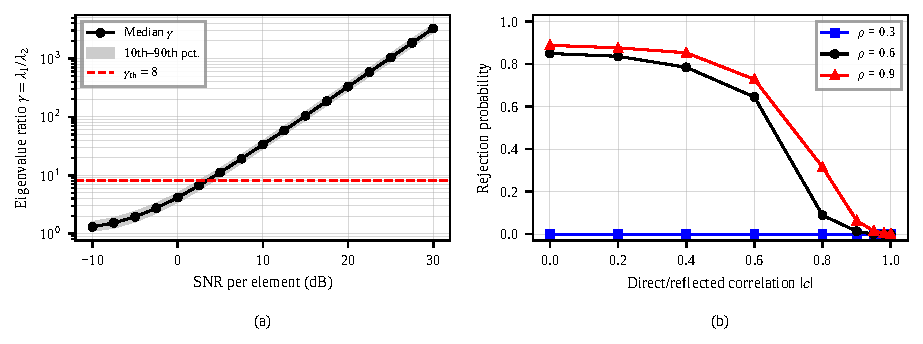
\includegraphics[width=0.90\textwidth]{figs/fig_gate.pdf}
\caption{Eigenvalue gate behavior at 915~MHz. (a) Eigenvalue ratio of clean bursts versus SNR. (b) Probability of rejection at 15~dB versus the direct/reflected correlation $|c|$ for three reflection strengths $\rho$.}
\label{fig:gate}
\end{figure*}
Fig.~\ref{fig:gate}(a) shows that the median $\gamma$ of clean bursts follows $M\Gamma+1$ from Eq.~(\ref{eq:gate}): 100\% of clean bursts are rejected at $\Gamma\le0$~dB, 94.8\% at 2.5~dB, but only 0.2\% at 5~dB and none above. The gate is therefore also an SNR gate. Fig.~\ref{fig:gate}(b) and Table~\ref{tab:gate} show its multipath behavior. A weak reflection ($\rho=0.3$, $-10.5$~dB) is never flagged, consistent with $\gamma\approx1/\rho^2\approx11>8$ from Eq.~(\ref{eq:gamma}). A $\rho=0.6$ reflection is flagged in 85\% of bursts when decorrelated, but only 9\% at $|c|=0.8$ and 0\% at $|c|=1$. A fully coherent specular reflection yields a $13^\circ$ error that the gate cannot see. The digital twin realization in Fig.~\ref{fig:dashboard}(d) illustrates this sharp discrimination between clean line-of-sight ($\lambda_1/\lambda_2 = 116.8$) and building reflections ($\lambda_1/\lambda_2 = 1.7$).


\begin{table}[!t]
\caption{Multipath Scenarios at 15~dB: Rejection Rate and DoA RMSE (Deg). Last Column: $P(\text{error}>5^\circ)$ for All/Accepted Bursts}
\label{tab:gate}
\centering
\footnotesize
\setlength{\tabcolsep}{3pt}
\begin{tabular}{@{}lcccccc@{}}
\toprule
Scenario & Rej. & MUSIC & Bart. & Capon & MUSIC (acc.) & $P_{>5^\circ}$ \\
\midrule
LoS only & 0\% & 0.5 & 0.5 & 0.5 & 0.5 & 0.00/0.00 \\
$\rho{=}0.3,\ |c|{=}0.5$ & 0\% & 3.6 & 3.5 & 1.8 & 3.6 & 0.17/0.17 \\
$\rho{=}0.6,\ |c|{=}0$ & 85\% & 6.4 & 5.8 & 2.0 & 9.6 & 0.43/0.94 \\
$\rho{=}0.6,\ |c|{=}0.6$ & 64\% & 9.8 & 9.0 & 2.9 & 12.2 & 0.56/0.75 \\
$\rho{=}0.9,\ |c|{=}0.6$ & 75\% & 50.2 & 48.9 & 46.6 & 59.8 & 0.80/1.00 \\
$\rho{=}0.6,\ |c|{=}1$ & 0\% & 13.1 & 13.1 & 13.2 & 13.1 & 0.70/0.70 \\
\bottomrule
\end{tabular}
\end{table}

Importantly, gating does not reduce the RMSE of the bursts it accepts (for example $9.6^\circ$ versus $6.4^\circ$ for $\rho=0.6$, $c=0$). The accepted bursts are those in which the two paths happen to be strongly correlated over the short burst, so $P(\text{error}>5^\circ)$ rises from 0.43 to 0.94. The gate is thus a detector of decorrelated multipath and low SNR, not an accuracy enhancer; a spatial-smoothing step \cite{shan} or a manifold-residual test would be needed for coherent reflections.


\subsection{Tracking}
\begin{figure*}[!t]
\centering
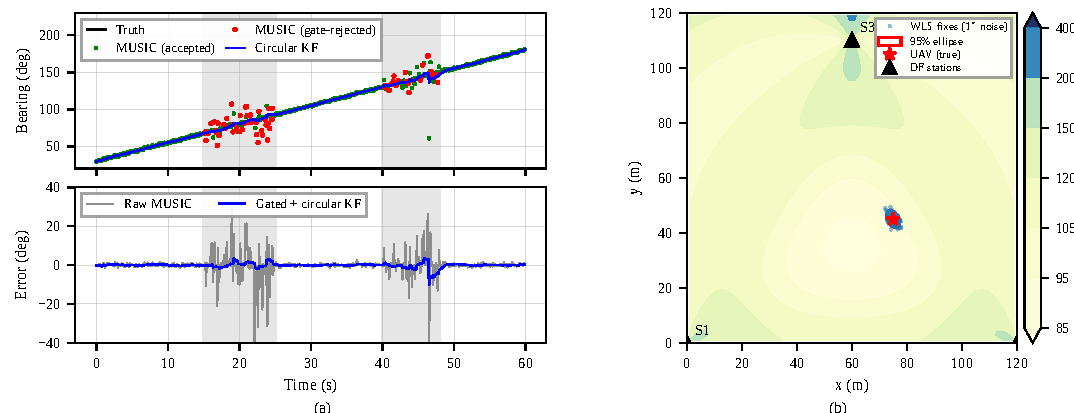
\includegraphics[width=0.90\textwidth]{figs/fig_trkgdop.pdf}
\caption{(a) Bearing tracking of a UAV moving at $2.5^\circ$/s with 10~Hz updates; shaded intervals are urban shadow zones with multipath (top: bearings, bottom: errors). (b) GDOP map of the three-station layout with 2000 WLS fixes (400 shown) and the 95\% confidence ellipse around the true UAV position.}
\label{fig:trk}
\end{figure*}
We simulated a 60~s bearing sweep at 10~Hz with SNR 12~dB and two urban shadow intervals in which 60\% of bursts carry a reflection ($\rho\in[0.4,0.9]$, $|c|\in[0,0.9]$). Table~\ref{tab:track} gives the RMSE over 40 runs. The circular Kalman filter reduces the error from $6.5^\circ$ to $1.9^\circ$ (Fig.~\ref{fig:trk}(a) and Fig.~\ref{fig:dashboard}(a)). Skipping rejected updates gives no additional benefit ($2.0^\circ$), in line with the selection effect above, so in this scenario the filtering rather than the gate provides the gain.

\begin{table}[!t]
\caption{Tracking RMSE (Degrees, Mean $\pm$ Std over 40 Runs)}
\label{tab:track}
\centering
\small
\begin{tabular}{@{}lc@{}}
\toprule
Method & RMSE \\
\midrule
Raw MUSIC (no filter) & 6.53 $\pm$ 1.99 \\
Gate + hold last bearing & 5.86 $\pm$ 2.56 \\
Circular KF, no gate & 1.91 $\pm$ 0.68 \\
Circular KF + gate & 2.04 $\pm$ 0.87 \\
\bottomrule
\end{tabular}
\end{table}

\subsection{Triangulation}
Three stations at (0,0), (120,0), and (60,110)~m localize a UAV at (75,45)~m with bearing noise of $1^\circ$ (Fig.~\ref{fig:trk}(b)). The Monte Carlo RMS position error is \trk~m, matching the \triTheory~m predicted from Eq.~(\ref{eq:gdop}). The GDOP at the target is \gdopT~m/rad, and its arena median is \gdopMed~m/rad; it grows near the baselines between stations.


%=====================================================================
\section{Hardware Roadmap}\label{sec:roadmap}
The mode-B prototype and its cost are in Table~\ref{tab:bom}. The total excludes the RTL-SDR receiver and a host computer.

\begin{table}[!t]
\caption{Proposed Prototype Bill of Materials (Mode B)}
\label{tab:bom}
\centering
\small
\begin{tabular}{@{}clp{3.4cm}r@{}}
\toprule
\# & Component & Function & Rs. \\
\midrule
1 & HMC241 / PE42440 & SP4T RF switch & 350 \\
2 & ESP32 NodeMCU & Switch timing control & 450 \\
3 & 4$\times$ monopole whips & UCA, $r=7.2$~cm & 500 \\
4 & RG316 and SMA leads & RF interconnect & 400 \\
\midrule
 & \multicolumn{2}{l}{Total (excluding SDR and PC)} & 1{,}700 \\
\bottomrule
\end{tabular}
\end{table}

The roadmap has three phases. \textbf{Phase~1} integrates the switch: the whips are mounted on a circular ground plane and the control lines are driven from ESP32 timer interrupts. \textbf{Phase~2} calibrates phase: fixed cable and port offsets are measured with a vector signal source and stored in a lookup table in EEPROM. \textbf{Phase~3} runs outdoor trials against authorized sub-GHz telemetry transmitters. The main risk is timing: the simulation assumes sample-synchronous switching, but an ESP32 timer is not locked to the SDR clock, so guard intervals or a pilot tone may be needed.

%=====================================================================
\section{Limitations and Conclusion}\label{sec:conclusion}
\textbf{Limitations.} All results are simulated. The channel is a two-path model with a correlation parameter rather than a ray-traced scene, burst detection is not stressed, the array is ideal (no mutual coupling), and a single UAV is assumed. The conclusions on the gate depend on the assumed path correlation, which must be measured in the field trials.

\textbf{Conclusion.} We presented and validated a frequency-aware DSP pipeline for a single-receiver switched UCA. Simulation shows that de-rotation with lag-$M$ refinement is the key enabler: it brings the switched array to the performance of an ideal coherent receiver and the CRB at SNR $\ge5$~dB, while static-wavelength steering is a minor penalty for the compact 7.2~cm array but fails beyond about 12~cm radius. The eigenvalue gate reliably rejects low-SNR and decorrelated-multipath bursts but cannot detect coherent reflections. Future work includes hardware calibration and field trials, coherent-multipath handling, and ESPRIT-class estimators for larger arrays.

\section*{Acknowledgment}
The authors thank IIIT Vadodara -- International Campus Diu and Dr.\ Varun Kumar for academic and infrastructure support.

\begin{thebibliography}{10}
\bibitem{schmidt} R. O. Schmidt, ``Multiple emitter location and signal parameter estimation,'' \emph{IEEE Trans. Antennas Propag.}, vol. AP-34, no. 3, pp. 276--280, Mar. 1986.
\bibitem{roy} R. Roy and T. Kailath, ``ESPRIT---Estimation of signal parameters via rotational invariance techniques,'' \emph{IEEE Trans. Acoust., Speech, Signal Process.}, vol. 37, no. 7, pp. 984--995, Jul. 1989.
\bibitem{vantrees} H. L. Van Trees, \emph{Optimum Array Processing: Part IV of Detection, Estimation, and Modulation Theory}. New York, NY, USA: Wiley, 2002.
\bibitem{stoica} P. Stoica and A. Nehorai, ``MUSIC, maximum likelihood, and Cram\'er--Rao bound,'' \emph{IEEE Trans. Acoust., Speech, Signal Process.}, vol. 37, no. 5, pp. 720--741, May 1989.
\bibitem{kay} S. M. Kay, ``A fast and accurate single frequency estimator,'' \emph{IEEE Trans. Acoust., Speech, Signal Process.}, vol. 37, no. 12, pp. 1987--1990, Dec. 1989.
\bibitem{fitz} M. P. Fitz, ``Further results in the fast estimation of a single frequency,'' \emph{IEEE Trans. Commun.}, vol. 42, no. 2--4, pp. 862--864, Feb.--Apr. 1994.
\bibitem{shan} T.-J. Shan, M. Wax, and T. Kailath, ``On spatial smoothing for direction-of-arrival estimation of coherent signals,'' \emph{IEEE Trans. Acoust., Speech, Signal Process.}, vol. ASSP-33, no. 4, pp. 806--811, Aug. 1985.
\bibitem{torrieri} D. J. Torrieri, ``Statistical theory of passive location systems,'' \emph{IEEE Trans. Aerosp. Electron. Syst.}, vol. AES-20, no. 2, pp. 183--198, Mar. 1984.
\bibitem{yee} K. S. Yee, ``Numerical solution of initial boundary value problems involving Maxwell's equations in isotropic media,'' \emph{IEEE Trans. Antennas Propag.}, vol. AP-14, no. 3, pp. 302--307, May 1966.
\bibitem{itu833} ITU-R, ``Attenuation in vegetation,'' Recommendation ITU-R P.833-9, Int. Telecommun. Union, Geneva, Switzerland, 2016.
\bibitem{elrs} ExpressLRS Project, ``ExpressLRS documentation.'' [Online]. Available: \url{https://www.expresslrs.org}
\end{thebibliography}
\end{document}
